\section{Visual Odometry}

Visual Odometry is the process of finding the position and orientation of a robot by analyzing the changes the motion induces on the images of the onboard cameras. It thus intends to find the change in position and rotation of a robot from the \((k)^{th}\) to the \((k+1)^{th}\) image. The result of the visual odometry algorithm is thus a composite translation and rotation matrix, denoted as \(RT\), which can be decomposed to their constituent translation \(T\) and rotation \(R\) matrices, and integrated over several such image pairs to produce an estimate of the state of the robot.

The main advantages of Visual odometry over conventional methods like wheel odometry are :

\begin{itemize}
  \item Not affected by wheel slip in uneven terrain, rainy/snowy weather or other adverse weather conditions.
  \item More accurate trajectory estimates are provided.
\end{itemize}


% Flowchart
\begin{figure}[H]
    \centering
    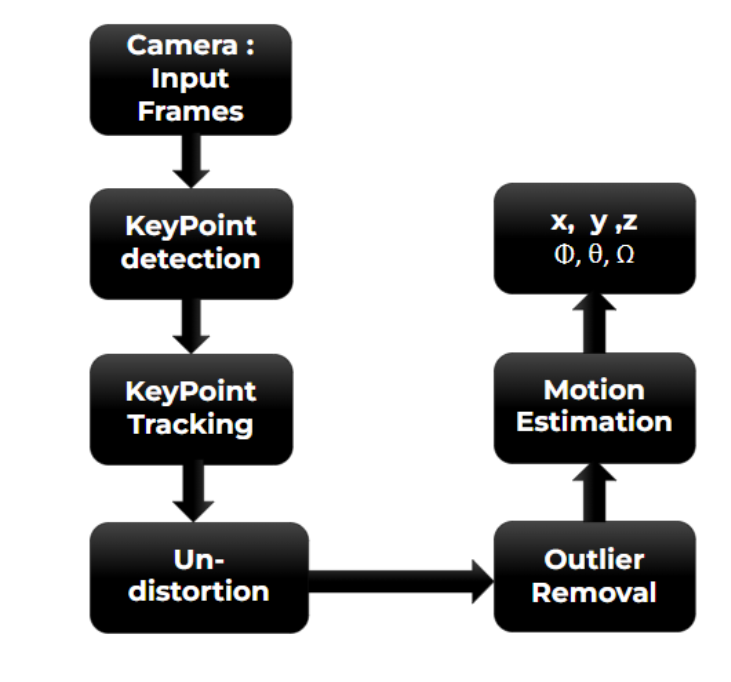
\includegraphics[width=0.9\textwidth]{vo}
    \caption{Flowchart}
    \label{fig:Visual Odometry}
\end{figure}

% Algorithm
\begin{algorithm}[hbt!]
    \caption{Visual odometry algorithm}\label{alg:cap}
    
    \begin{algorithmic}[1]
    
        \Require $img \gets Image\ data\ from\ stereo\ camera$
        \State $Apply\ KeyPoint\ detection\ algorithm\ to\ detection\ $
        \State $Apply\ KeyPoint\ tracking\ algorithm\ $
        \State $Undistortion\ is\ performed\ on\ the\ image\ $
        \State $Perform\ outlier\ removal\ $
        \\
        \Return $Pose$
        
    \end{algorithmic}
\end{algorithm}

\begin{figure}[H]
  \centering
    \begin{multicols}{2}
        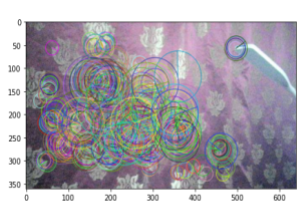
\includegraphics[width=0.5\textwidth]{feature_Detection}
        \caption{Feature Detection}
        \label{fig:Feature Detection}
        
        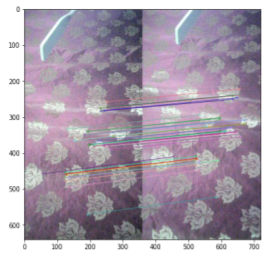
\includegraphics[width=0.5\textwidth]{feature_matching}
        \caption{Feature Matching}
        \label{fig:Feature Matching}
    \end{multicols} 
    
    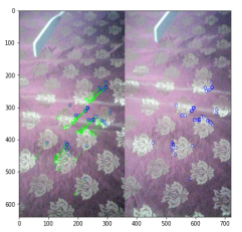
\includegraphics[width=0.5\textwidth]{motion_estimation}
        \caption{Motion Estimation}
        \label{fig:Motion Estimation}
    
\end{figure}

 